\makeatletter
\def\input@path{{../../}}
\makeatother
\documentclass[../../main.tex]{subfiles}

\graphicspath{
	{../../img/}
	{../img/}
	{img/}
}

\begin{document}
\subsection{КрИ-1 в $\R^3$}

Если $\overbow{AB}$~--- пространственная кривая, то по той же схеме,
что и в $\R^2$, вводится КрИ-1 по $\overbow{AB}$:
\[
\int\limits_{\tiny{\overbow{AB}}} f(x,\, y,\, z)\, ds.
\]
В этом случае на $\overbow{AB}$ определена функция от трех переменных.

Если $\overbow{AB}$ задана в естественной параметризации, то:

\begin{equation}
\label{lec_19, num_1}
\int\limits_{\tiny{\overbow{AB}}} f(x,\, y,\, z)\, ds = \left[
\overbow{AB}: 
\begin{cases}
x = x \left( s \right),\\
y = y \left( s \right),\\
z = z \left( s \right),\\
a \leq s \leq b 
\end{cases} \right] = 
\int\limits_{a}^{b} f(x \left( s \right),\, y \left( s \right),\, z \left( s 
\right))\, ds.
\end{equation}

Если $\overbow{AB}$ задана в произвольной параметризации, то
\begin{equation}
\label{lec_19, num_2}
\begin{gathered}
\int\limits_{\tiny{\overbow{AB}}} f(x,\, y,\, z)\, ds = \left[
\overbow{AB}: 
\begin{cases}
x = x \left( t \right),\\
y = y \left( t \right),\\
z = z \left( t \right),\\
\alpha \leq t \leq \beta 
\end{cases} \right] =
\\
= \int\limits_{\alpha}^{\beta} 
f(x \left( t \right),\, y \left( t \right),\, z \left( t \right))
\sqrt{ \left( x'(t) \right)^2 + \left( y'(t) 
\right)^2 + \left( z'(t) \right)^2}\, dt.
\end{gathered}
\end{equation}

По аналогичной схеме приводят аналогичные формулы.

\begin{example}
Вычислим $\displaystyle \int\limits_{\tiny{\overbow{AB}}} (x^2 + y^2)\, ds,\  
\overbow{AB}:
\begin{cases}
x = a \cos{t},\\
y = a \sin{t},\\
z = b t,\\
0 \leq t \leq 2\pi. 
\end{cases}
$

\begin{enumerate}

\item
По формуле \eqref{lec_19, num_2} имеем:
\begin{gather*}
I = \int\limits_{0}^{2\pi} \left(a^2 \cos^2{t} + a^2 \sin^2{t}\right)
 \sqrt{a^2 \sin^2{t} + a^2 \cos^2{t} + b^2}\, dt =
\\
= \int\limits_{0}^{2\pi} a^2
 \sqrt{a^2 + b^2}\, dt = 2\pi a^2 \sqrt{a^2 + b^2}. 
\end{gather*}

\begin{center}
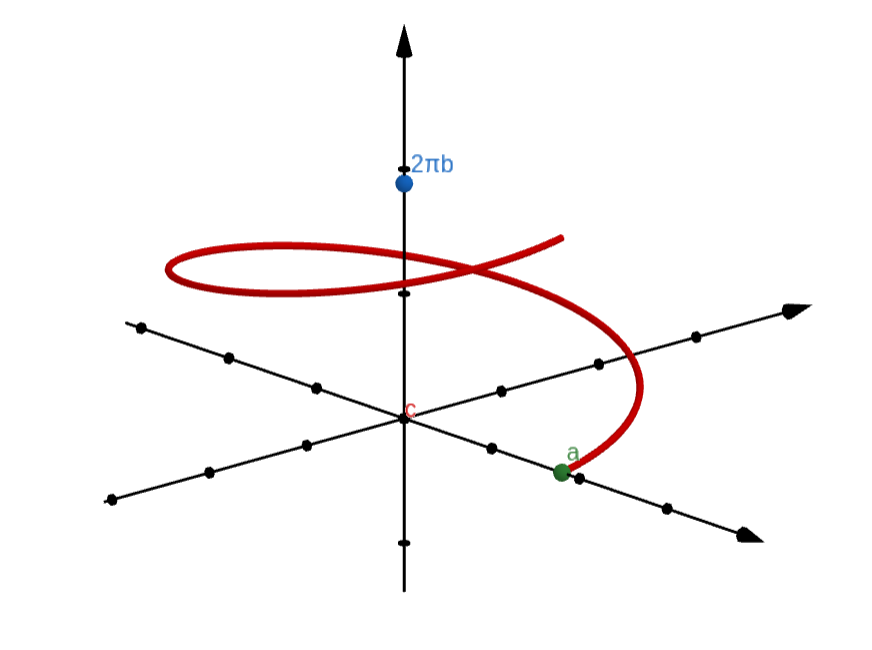
\includegraphics[scale = 0.4]{lec19_1.png}
\end{center}

\item
Попробуем задать эту кривую в естественной параметризации:
\[s = \text{длина }\overbow{A(0), A(t)} = 
\int\limits_{0}^{t} \sqrt{\left( x'(t) \right)^2 + \left( y'(t) 
\right)^2 + \left( z'(t) \right)^2}\, dt = 
t \sqrt{a^2 + b^2} \implies
\]
\[ \implies t = \frac{s}{\sqrt{a^2 + b^2}} \implies 
\overbow{AB}:
\begin{cases}
x = a \cos{\frac{s}{\sqrt{a^2 + b^2}}},\\
y = a \sin{\frac{s}{\sqrt{a^2 + b^2}}},\\
z = b \frac{s}{\sqrt{a^2 + b^2}}.\\
\end{cases}
\]

При этом, если $t = 2 \pi$, то получим точку $B$, и $s = l = 2 \pi 
\sqrt{a^2 + b^2}$.
Тогда, воспользовавшись формулой \eqref{lec_19, num_1}, имеем:
\[
I = \int\limits_{0}^{2 \pi \sqrt{a^2 + b^2}} a^2\, ds = 2\pi a^2 \sqrt{a^2 + 
b^2}.
\]
\end{enumerate}
\end{example}

\section{Криволинейный интеграл второго рода (КрИ-2)}

\subsection{КрИ-2 в $\R^2$}

Пусть $\overbow{AB}$~--- гладкая кривая в $\R^2$, на которой задано 
направление (ориентированная кривая). 
Пусть на $\overbow{AB}$ заданы функции $P \left( x,\, y \right),\, Q \left( 
x,\, y \right)$.
Разобьём $\overbow{AB}$ точками $A_k \left( x_k,\, y_k \right),\ k = 
\overline{0,n}$.
Тогда $\Delta x_k = x_k - x_{k - 1},\ \Delta y_k = y_k - y_{k - 1}$.
На каждой дуге $\overbow{A_{k - 1} A_{k}}$ возьмём произвольную точку 
$M_k(\widetilde{x_k},\, \widetilde{y_k})$.

Составим интегральные суммы:
\[
\begin{cases}
\sigma_1 = \sum\limits_{k = 1}^{n} P \left( \widetilde{x_k},\, \widetilde{y_k}
\right) \Delta x_k,\\
\sigma_2 = \sum\limits_{k = 1}^{n} Q \left( \widetilde{x_k},\, \widetilde{y_k} 
\right) \Delta y_k.
\end{cases}
\]

Пусть $\delta$~--- диаметр разбиения, то есть
$\delta = \max{\text{дл. } \overbow{A_{k - 1} A_k}}$. Тогда пределы 
интегрирования
\[
\begin{gathered}
\lim\limits_{\delta \to 0} \sigma_1 = \int\limits_{\tiny{\overbow{AB}}} P 
\left( x,\, 
y \right) dx,\\
\lim\limits_{\delta \to 0} \sigma_2 = \int\limits_{\tiny{\overbow{AB}}} Q 
\left( x,\, 
y \right) dy,
\end{gathered}
\]
называют \emph{криволинейными интегралами второго рода} (КрИ-2) по 
ориентированной кривой $\overbow{AB}$.

Рассматривают также КрИ-2 общего вида:
\[
\int\limits_{\tiny{\overbow{AB}}} P\left(x,\, y \right)\, dx + Q\left(x,\, y 
\right)\, dy.
\]

Если $\overbow{AB}$ является гладкой кривой, а
функции $P(x, y)$ и $Q(x, y)$ непрерывны и ограниченны, 
то эти интегралы существуют.

\subsection{Физический смысл КрИ-2}

Представим, что на $\overbow{AB}$ находится точка с массой $m = 1$.
В каждой точке кривой определён вектор силы $\vec{F}(x, y)$ с 
координатами $\vec{F} ( x, y ) = \left( P ( x, 
y ), Q ( x, y ) \right)$.
На элементе кривой, то есть на дуге $\overbow{A_{k-1}A_k}$
(при достаточно малом разбиении ее можно заменить хордой) 
элементарная работа силы $F$ будет равна:
\[
\Delta_k A \approx \left| \overrightarrow{F} \right| \cdot \left| 
\overrightarrow{A_{k - 1} A_k} \right| \cdot \cos{\alpha} =
\langle \overrightarrow{F}, \overrightarrow{A_{k - 1}, A_{k}} \rangle = 
\langle \left( P,\, Q \right), \left( \Delta x_k,\, \Delta y_k \right) \rangle 
= P \Delta x_k + Q \Delta y_k.
\]

Суммируя элементарные работы, мы получим приближённо работу 
$\overrightarrow{F}$ на $\overbow{AB}$:
\[
A \approx \sum\limits_k P \left( \widetilde{x_k},\, \widetilde{y_k} \right) 
\Delta x_k + Q \left( \widetilde{x_k},\, \widetilde{y_k} \right) \Delta y_k.
\]
Переходя к пределу при $\delta \to 0$, получим:
\[
A = \int\limits_{\tiny{\overbow{AB}}} P \left( x,\, y \right)\, dx + Q \left( 
x,\, y 
\right) dy.
\] 

\subsection{Вычисление КрИ-2}

Пусть $\overbow{AB}$~--- гладкая ориентированная кривая,
заданная уравнениями
\[
\overbow{AB}:
\begin{cases}
x = x \left( t \right),\\
y = y \left( t \right),\\
\alpha \leq t \leq \beta.
\end{cases}
\]
Это равносильно заданию векторного вида такой кривой:
\[
\overrightarrow{r} = \overrightarrow{r}(t) =
\left( x \left( t \right),\, y \left( t \right) \right),\ 
\alpha \leq t \leq \beta.
\]

Т.~к. кривая гладкая, то $x(t)$, $y(t)$ имеют непрерывные производные. При 
этом 
каждой точке разбиения $A_k$ соответствует значение $t_k$. Тогда:
\[
\Delta x_k = x \left( t_k \right) - x \left( t_{k - 1} \right) = \left[ 
\text{формула Лагранжа} \right] =
x' \left( \overline{t_k} \right) \Delta t_k,
\]
где $\overline{t_k}$~--- некоторая точка из $\left[ t_{k - 1}, t_k \right]$.

Пусть $M_k(\widetilde{x_k}, \widetilde{y_k})$ 
соответствует $\widetilde{t_k}$, тогда:
\[
\sigma_1 = \sum\limits_{k = 1}^{n} P \left( \widetilde{x_k},\, \widetilde{y_k} 
\right) \Delta x_k =
\sum\limits_{k = 1}^{n} P \left( \widetilde{x_k},\, \widetilde{y_k} \right) x' 
\left( \overline{t_k} \right) \Delta t_k = *
\]
Как и в рассуждениях для КрИ-1 (см. \ref{subsec:kri1-eval}), имеем
$x' \left( \overline{t_k} \right) \Delta t_k = \left( x' \left( 
\widetilde{t_k} \right) + \alpha_k \right) \Delta t_k$,
причем $\alpha_k \appr{\delta \to 0} 0$ 
в силу равномерной непрерывности и формулы Лагранжа. Тогда
\[ 
* = \sum\limits_{k = 1}^{n} P \left( \widetilde{x_k},\, \widetilde{y_k} 
\right) x' \left( \widetilde{t_k} \right) \Delta t_k +
\underbrace{\sum\limits_{k = 1}^{n} P \left( \widetilde{x_k},\, 
\widetilde{y_k} \right) 
\alpha_k \Delta t_k}_{\alpha},\ \alpha \appr{\delta \to 0} 0.
\]
Пусть $\delta \to 0$. Cлева~--- интегральная сумма для КрИ-2, а справа~--- 
интегральная сумма для 1И на отрезке $\left[\alpha, \beta\right]$ с разбиением 
$t_k$ и промежуточными точками $\widetilde{t_k}$. Таким образом, получаем:
\[
\int\limits_{\tiny{\overbow{AB}}} P \left( x,\, y \right)\, dx = 
\int\limits_\alpha^{\beta} P \left( x(t),\, y(t) \right) \cdot x' \left( t 
\right)\, dt. 
\] 
Аналогично для $Q$ получаем:
\[
\int\limits_{\tiny{\overbow{AB}}} Q \left( x,\, y \right)\, dy = 
\int\limits_\alpha^{\beta} Q \left( x(t),\, y(t) \right) \cdot y' \left( t 
\right)\, dt. 
\]
Тогда КрИ-2 общего вида приобретает вид:

\begin{equation}
\label{lec_19, num_3}
\int\limits_{\tiny{\overbow{AB}}} P \left( x,\, y \right)\, dx + Q \left( x,\, 
y 
\right)\, dy =
\int\limits_{\alpha}^{\beta} \left( P(x(t),y(t)) \cdot x' \left( t \right)
+ Q(x(t),y(t)) \cdot y' \left( t 
\right) \right)\, dt. 
\end{equation}

\begin{exmp}
\label{indep-int}

Вычислим $\displaystyle\int\limits_{\tiny{\overbow{AB}}} 2 x y\, dx + x^2\, 
dy$, где $A = (0, 
0)$, $B 
= (1, 1)$.

\begin{itemize}

	\item[а)] $AB$~--- отрезок.

	По формуле \eqref{lec_19, num_3}:
	\[
	I = \left[ AB:	
	\begin{cases}
	x = t,\\
	y = t,\\
	0 \leq t \leq 1
	\end{cases}
	\right] = 
	\int\limits_{0}^{1} 2 t^{2} \cdot 1 + t^{2} \cdot 1\, dt = 
	\int\limits_{0}^{1} 3 t^{2}\, dt = 1.
	\]

	\item[б)] $y = x^{2}$.

	\[
	I = \left[ AB:	
	\begin{cases}
	x = t\\
	y = t^{2}\\
	0 \leq t \leq 1
	\end{cases}
	\right] = 
	\int\limits_{0}^{1} \left(2 t^{3} + 2 t^{3}\right)\, dt = 
	\int\limits_{0}^{1} 4 t^{3}\, dt = 1.
	\]

	\item[в)] $y = x^{10}$.

	\[
	I = \left[ AB:	
	\begin{cases}
	x = t\\
	y = t^{10}\\
	0 \leq t \leq 1
	\end{cases}
	\right] = 
	\int\limits_{0}^{1} \left(2 t^{11} + 10 t^{11}\right)\, dt = 
	\int\limits_{0}^{1} 12 t^{11}\, dt = 1.
	\]

\end{itemize}

	Нетрудно показать, что вне зависимости от степени $x$ ответ всегда будет равен
	$1$.

\end{exmp}

\subsection{Свойства КрИ-2}

\begin{enumerate}[label=\arabic*$^{\circ}$]
	\item $\displaystyle\int\limits_{\tiny{\overbow{AB}}} = 
	-\int\limits_{\tiny{\overbow{BA}}}$.

	Свойство следует из того, что $\Delta x_k = x_k - x_{k - 1}, \, \Delta y_k = 
	y_k 
	- y_{k - 1}$
	при смене направлении меняют знак.
	\item Линейность (по аналогии с 1И).
	\item Аддитивность (по аналогии с 1И).
	\item Основная оценка:

	Если $\left| P \left( x,\, y \right) \right| \leq M\quad \forall \left( 
	x,\, y \right) \in \overbow{AB}$,
	то $\displaystyle\abs{\int\limits_{\tiny{\overbow{AB}}} P \left( x,\, y 
	\right)\, dx} \leq M 
	\cdot l.$

	Для доказательства достаточно оценить интегральную сумму $\sigma_1$.
\end{enumerate}

\subsection{КрИ-2 в $\R^3$}

	Если $\overbow{AB}$~--- гладкая пространственная кривая, на которой 
	определены функции
	$P \left( x,\, y,\, z \right)$, $Q \left( x,\, y,\, z \right)$, $R \left( 
	x,\, y,\, z \right)$,
	то по аналогии с КрИ-2 в $\R^2$ определяют КрИ-2 в $\R^3$:
	\[I = 
	\int\limits_{\tiny{\overbow{AB}}} P \left( x,\, y,\, z \right)\, dx + Q 
	\left( x,\, 
	y,\, z \right)\, dy + R \left( x,\, y,\, z \right)\, dz. 
	\]

	КрИ-2 в $\R^3$ обладает теми же свойствами, что и КрИ-2 в $\R^2$.

	Если $\overbow{AB}$ задана в произвольной параметризации:
	\[
	\overbow{AB}:
	\begin{cases}
	x = x \left( t \right),\\
	y = y \left( t \right),\\
	z = z \left( t \right),\\
	\alpha \leq t \leq \beta
	\end{cases}
	\] 
	или в векторном виде
	\[
	\overrightarrow{r} = \overrightarrow{r} \left( t \right) = \left( x \left( t 
	\right),\, y \left( t \right),\, z \left( t \right) \right),\ 
	\alpha \leq t \leq \beta,
	\]
	то КрИ-2 в $\R^3$ принимает вид
	\begin{equation}
	\label{lec_19, num_4}
	I = \int\limits_{\alpha}^{\beta} P \left( x \left( t \right),\, y \left( t 
	\right),\, z \left( t \right) \right)\, dx +
	Q \left( x \left( t \right),\, y \left( t \right),\, z \left( t \right) 
	\right)\, dy +
	R \left( x \left( t \right),\, y \left( t \right),\, z \left( t \right) 
	\right)\, dz. 
	\end{equation}
	
	\begin{example}
	Вычислить $\displaystyle 
	\int\limits_{\tiny{\overbow{AB}}} yz\, dx + xz\, dy + xy\, dz,\  
	\overbow{AB}:
	\begin{cases}
	x = t,\\
	y = t^2,\\
	z = t^3,\\
	0 \leq t \leq 1.
	\end{cases}$
	\[
	I = \int\limits_{0}^{1} \left( t^5 \cdot 1 + t^4 \cdot 2t + t^3 \cdot 3t^2 
	\right)\, dt = \int\limits_{0}^{1} 6 t^5\, dt = 1.
	\]
	\end{example}	 

\end{document}
